\section{Einführung}
Eine reale Spannungsquelle wird durch das Modell des Innenwiderstandes beschrieben. Dabei wird gerechnet, als wäre ein Innenwiderstand $R_i$ in Reihe mit der eigentlichen Spannungsquelle mit Leerlaufspannung $U_0$ geschaltet. Es ergibt sich bei Belastung durch einen Außenwiderstand $R_a$ (Strom $I$):
\begin{equation}
  U_0=R_i\cdot I+R_a\cdot I
  \label{eq:innenwiderstand}
\end{equation}
Die tatsächlich gemessene Spannung an der Quelle weicht von der Leerlaufspannung ab und heißt Klemmspannung $U_{\text{Kl}}$:
\begin{equation}
  U_{\text{Kl}}=U_0-R_i\cdot I=R_a\cdot I
  \label{eq:klemmspannung}
\end{equation}
Beim Kurzschluss für $R_a=0$ fließt der endliche Strom
\begin{equation}
  I_{\text{Ks}}=U_0/R_i.
  \label{eq:kurzschluss}
\end{equation}
Die an den Verbraucher abgegebene Leistung beträgt
\begin{equation}
  P=U_0^2 \frac{R_a}{(R_a+R_i)^2}.
  \label{eq:leistung}
\end{equation}
Wir leiten die Bedingung für maximale Leistungsabgabe her:
\begin{align}
  &\frac{\mathrm{d}P}{\mathrm{d}R_a}=\frac{U_0^2}{(R_a-R_i)^2}-2\cdot \frac{R_a U_0^2}{(R_a+R_i)^3}=0 \\
  &\implies (R_a+R_i)=2R_a \implies R_a=R_i
  \label{eq:maxleistung}
\end{align}
Bei Wechselstrom wird keine konstante Spannung angelegt, sondern eine Periodisch veränderliche. In der Regel entspricht der Spannungsverlauf einer (Ko-)Sinusfunktion, jedoch sind auch andere Verläufe möglich. 
\begin{equation}
	U = U(t) = U_0 \sin(\omega t + \varphi_U)
\end{equation}
Die Stromstärke ist nur bei Ohmschen Widerständen direkt proportional zur Spannung. Bei Spule und Kondensator kommt es dagegen zu einer Phase $ \varphi = \varphi_U - \varphi_I $ zwischen Spannung und Strom.
\begin{align}
	&\text{Ohmscher Widerstand } R & U_R = R I&,~\varphi = 0 \\
	&\text{Spule mit Induktivität } L & U_L = L \frac{\di I}{\di t}&,~\varphi= \frac{\pi}{2} \\
	&\text{Kondensator mit Kapazität } C & U_C = \frac{1}{C} \int I \di t&,~\varphi = -\frac{\pi}{2}
\end{align}
Die Leistung bleibt das Produkt aus Spannung und Stromstärke. Jedoch ist meistens nur der Mittelwert von Interesse. Für Gleichstrom ergibt das
\begin{equation}
	\bar{P} = \frac{1}{T} \int_{t_0}^{t_0+T} P(t) \di t = \frac{1}{T} \int_{0}^{T} U_0 I_0 \sin^2(\omega t) \di t = \frac{U_0}{\sqrt{2}} \frac{I_0}{\sqrt{2}}
\end{equation}
Daher Definiert man die Effektivwerte 
\begin{equation}
	U_{eff} = \frac{U_0}{\sqrt{2}} \qquad\qquad I_{eff} = \frac{I_0}{\sqrt{2}}
\end{equation}
Im allgemeinen gilt
\begin{equation}
	\bar P = U_{eff}I_{eff} \cos \varphi \label{eq:phase}
\end{equation}
Um Wechselstrom zu messen sind Messgeräte oft zu träge. Dann erhält man den linearen Mittelwert
\begin{equation}
	A = \frac{1}{T} \int_{t_0}^{t_0 + T} A(t) \di t 
\end{equation}
Bei Sinuswellen ist dies $ 0 $. Daher wird stattdessen der Gleichspannungsteil, bzw. der Effektivwert verwendet 
\begin{align}
	A_= &= \frac{1}{T} \int_{t_0}^{t_0 + T} |A(t)| \di t \\
	A_{eff} &= \sqrt{\frac{1}{T} \int_{t_0}^{t_0 + T} \big(A(t)\big)^2 \di t} 
\end{align}
Bei sinusförmigen Wechselstrom ergibt sich
\begin{align}
	I_{=} &= \frac{1}{T}\int_{0}^{T}|I_{0}\sin(\omega t)| \di t=I_{0}\frac{2}{T}\int_{0}^{\frac{T}{2}}\sin(\omega t) \di t = \frac{2}{\pi} I_0 \\
	I_{eff}&=\sqrt{\frac{1}{T}\int_{0}^{T}I_{0}^{2}\sin^{2}(\omega t)\di t}=\sqrt{\frac{I_{0}^{2}}{2T}\int_{0}^{T}(1-\cos(2\omega t))\di t}=\frac{|I_{0}|}{\sqrt{2}}
\end{align}
Mit Widerständen rechnet man bei Wechselstrom mittels Scheinwiderständen. Zusammen mit der Phase lässt sich die Stromstärke in Abhängigkeit von der Zeit berechnen. Allgemein gilt
\begin{equation}
	|Z| = \frac{U_{eff}}{I_{eff}}
\end{equation} Für ohmschen Widerstand, Spule und Kondensator sind Scheinwiderstand und Phase
\begin{align}
	&\text{Ohmscher Widerstand } R & |Z|_{R} = R &,~\varphi = 0 \label{eq:Rohm} \\
	&\text{Spule mit Induktivität } L & |Z|_{L} = \omega L &,~\varphi= \frac{\pi}{2} \\
	&\text{Kondensator mit Kapazität } C & |Z|_{C} = \frac{1}{\omega C} &,~\varphi = -\frac{\pi}{2}
\end{align}
Da im Phasenraum $ Z_{R} $ senkrecht zu $ Z_{L} $ und $ Z_{C} $ ist, ist der Gesamtscheinwiderstand bei Reihenschaltung gegeben durch
\begin{equation}
	|Z| = \sqrt{|Z|_{R}^2 + (|Z|_{L} - |Z|_{C})^2}~,\qquad \tan\varphi = \frac{R_{W,L} - R_{W,C}}{R_{W,R}} \label{eq:Induk}
\end{equation}
Für den Wirkwiderstand gilt
\begin{equation}
	R_W = |Z| \cos\varphi = \frac{U_{eff}}{I_{eff}} \cos\varphi \label{eq:wirkohm}
\end{equation}
\section{Versuche}
\subsection{Aufgabe 1}
Ziel dieses Versuches ist die Bestimmung von Leerlaufspannung $U_0$ und Innenwiderstand $R_i$ von
\begin{enumerate}
  \item einer einzelnen Akkumulatorzelle
  \item drei Zellen parallel
  \item drei Zellen in Reihe.
\end{enumerate}
Dazu wird ein Stöpselwiderstand $R_a$ in Reihe und ein Spannungsmessgerät zur Messung der Klemmspannung $U_{\text{Kl}}$ parallel zu den Zellen geschaltet. Der Stöpselwiderstand fungiert als Lastwiderstand, über den der Strom $I$ reguliert werden kann. Es werden jeweils 13 Spannungswerte nach Einstellen verschiedener Widerstände $R_a$ abgenommen. Darunter sind auch Werte für den Kurzschlussfall ($R_a$=0) und für nicht geschlossenen Stromkreis ($R_a=\infty$).
\begin{table}[H]
  \centering
  \begin{tabular}{c c c} \toprule
    $R_a$ [\SI{\pm1}{\ohm}] & $U_{\text{Kl}}$ [\SI{\pm .015}{V}] & $I=U_{\text{Kl}}/R_a$ [\SI{\pm .5}{mA}] \\ \midrule
    $\infty$ & \num{1.338} & 0 \\
    0 & \num{0.021} & - \\
    5 & \num{0.303} & \num{60.6} \\
    10 & \num{.483} & \num{48.3} \\
    20 & \num{.717} & \num{35.8} \\
    30 & \num{.840} & \num{28.0} \\
    40 & \num{.930} & \num{23.3} \\
    50 & \num{.987} & \num{19.7} \\
    60 & \num{1.035} & \num{17.3} \\
    70 & \num{1.071} & \num{15.3} \\
    80 & \num{1.095} & \num{13.7} \\
    90 & \num{1.113} & \num{12.4} \\
    100 & \num{1.140} & \num{11.4} \\ \bottomrule
  \end{tabular}
  \caption{Messergebnis für eine Zelle}
  \label{tab:einezelle}
\end{table}

\begin{table}[H]
  \centering
  \begin{tabular}{c c c} \toprule
    $R_a$ [\SI{\pm 1}{\ohm}] & $U_{\text{Kl}}$ [\SI{\pm .05}{V}] & $I=U_{\text{Kl}}/R_a$ [\SI{\pm 1.2}{mA}] \\ \midrule
    $\infty$ & \num{4.00} & 0 \\
    0 & \num{0.10} & - \\
    5 & \num{0.40} & \num{80} \\
    10 & \num{.70} & \num{70} \\
    20 & \num{1.15} & \num{57.5} \\
    30 & \num{1.48} & \num{49.3} \\
    40 & \num{1.73} & \num{43.3} \\
    50 & \num{1.98} & \num{39.6} \\
    60 & \num{2.12} & \num{35.3} \\
    70 & \num{2.30} & \num{32.9} \\
    80 & \num{2.40} & \num{30.0} \\
    90 & \num{2.52} & \num{28.0} \\
    100 & \num{2.61} & \num{26.1} \\ \bottomrule
  \end{tabular}
  \caption{Messergebnis für drei Zellen parallel}
  \label{tab:einezelle}
\end{table}

\begin{table}[H]
  \centering
  \begin{tabular}{c c c} \toprule
    $R_a$ [\SI{\pm1}{\ohm}] & $U_{\text{Kl}}$ [\SI{\pm .015}{V}] & $I=U_{\text{Kl}}/R_a$ [\SI{\pm .5}{mA}] \\ \midrule
    $\infty$ & \num{1.323} & 0 \\
    0 & \num{0.030} & - \\
    5 & \num{0.327} & \num{65.4} \\
    10 & \num{.495} & \num{49.5} \\
    20 & \num{.717} & \num{35.9} \\
    30 & \num{.843} & \num{28.1} \\
    40 & \num{.930} & \num{23.3} \\
    50 & \num{.990} & \num{19.8} \\
    60 & \num{1.023} & \num{17.1} \\
    70 & \num{1.068} & \num{15.3} \\
    80 & \num{1.095} & \num{13.7} \\
    90 & \num{1.113} & \num{12.4} \\
    100 & \num{1.137} & \num{11.4} \\ \bottomrule
  \end{tabular}
  \caption{Messergebnis für drei Zellen in Reihe}
  \label{tab:einezelle}
\end{table}
Wir beobachten bei allen drei Messungen eine Zunahme der Klemmspannung $U_{\text{Kl}}$ und Abnahme des Stromes $I$ bei höherem Lastwiderstand $R_a$. Die Werte für eine Zelle entsprechen bis auf geringe Abweichungen den Werten für drei Zellen in Reihe. Die größte Abweichung tritt für $R_a=\SI{5}{\ohm}$ auf und beträgt $\Delta U_0=(\SI{0.327}{V}-\SI{0.303}{V})/(\SI{0.303}{V})\approx \SI{8}{\percent}$.\\

Aus \cref{eq:klemmspannung} erwarten wir einen linearen Zusammenhang zwischen Klemmspannung und Strom. Wir fitten also mit gnuplot nach dem \textit{least-squares}-Verfahren gegen $U_{\text{Kl}}(I)=U_0-R_i\cdot I$. Ausgabe:
\begin{table}[H]
  \centering
  \begin{tabular}{c c c} \toprule
    Messung & $U_0$ [\si{V}] & $R_i$ [\si{\ohm}] \\ \midrule
    1 Zelle & \num{1.33(1)} & \num{17.2(2)} \\
    3 Zellen parallel & \num{3.79(7)} & \num{44.9(16)} \\
    3 Zellen in Reihe & \num{1.30(1)} & \num{15.6(4)}
  \end{tabular}
  \caption{Klemmspannung und Innenwiderstand aus Fit}
  \label{tab:fita1}
\end{table}

\begin{figure}[H]
  \centering
  \begin{tikzpicture}
    \begin{axis}[
      width=15 cm,
      height=9 cm,
      xmin=-0.5, xmax=82,
      ymin=0, ymax=4.1,
      xlabel={Strom $I$ [\si{mA}]},
      ylabel={Klemmspannung $U_{\text{Kl}}$ [\si{V}]},
      legend entries={1 Zelle, 3 Zellen parallel, 3 Zellen in Reihe, $\num{1.33}-\num{0.0172}x$, $\num{3.79}-\num{0.0449}x$, $\num{1.30}-\num{0.0156}x$},
      legend pos=north east,
      domain=0:80,
    ]
    \addplot+[only marks,error bars/.cd, x dir=both, x fixed=0.5, y dir=both, y fixed=0.015]  file {1zelle.txt};
    \addplot+[only marks,error bars/.cd, x dir=both, x fixed=1.2, y dir=both, y fixed=0.05]  file {3zellen_parallel.txt};
    \addplot+[only marks,error bars/.cd, x dir=both, x fixed=0.5, y dir=both, y fixed=0.015]  file {3zellen_reihe.txt};
    \pgfplotsset{cycle list shift=-3};
    \addplot+[mark=none] {1.33-0.0172*x};
    \addplot+[mark=none] {3.79-0.0449*x};
    \addplot+[mark=none] {1.30-0.0156*x};
    \end{axis}
  \end{tikzpicture}
  \caption{Klemmspannung $U_{\text{Kl}}$ abhängig vom Strom $I$ mit eingezeichnetem Fit}
  \label{fig:fita1}
\end{figure}
\section{Aufgabe 2}
Anhang von \cref{eq:leistung} kann mithilfe der Werte für $U_0$, $R_i$ aus dem vorherigen Aufgabenteil die an den Verbraucher abgegebene Leistung $P$ berechnet werden.

\begin{figure}[H]
  \centering
  \begin{tikzpicture}
    \begin{axis}[
      width=12 cm,
      height=9 cm,
      xmin=4, xmax=101,
      ymin=10, ymax=100,
      xlabel={Außenwiderstand $R_a$ [\si{\ohm}]},
      ylabel={Leistung am Verbraucher $P$ [\si{mW}]},
      legend style={text height=3.4ex},
      legend entries={1 Zelle, 3 Zellen parallel, 3 Zellen in Reihe,$10^3\cdot \frac{R_a\cdot \SI{1.33}{V}}{(R_a+\SI{17.2}{\ohm})^2}$, $10^3\cdot \frac{R_a\cdot \SI{3.79}{V}}{(R_a+\SI{44.9}{\ohm})^2}$, $10^3\cdot \frac{R_a\cdot \SI{1.30}{V}}{(R_a+\SI{15.6}{\ohm})^2}$},
      legend pos=outer north east,                                  
      domain=5:100,                                                 
    ]
    \addplot+[only marks,table/y expr=1000*\thisrowno{0}*(1.33)^2/(\thisrowno{0}+17.2)^2, error bars/.cd, x dir=both, x fixed=0.5, y dir=both, y fixed=0.001]  table {widerstaende.txt};
    \addplot+[only marks,table/y expr=1000*\thisrowno{0}*(3.79)^2/(\thisrowno{0}+44.9)^2, error bars/.cd, x dir=both, x fixed=0.5, y dir=both, y fixed=0.001]  table {widerstaende.txt};
    \addplot+[only marks,table/y expr=1000*\thisrowno{0}*(1.30)^2/(\thisrowno{0}+15.6)^2, error bars/.cd, x dir=both, x fixed=0.5, y dir=both, y fixed=0.001]  table {widerstaende.txt};
    \pgfplotsset{cycle list shift=-3};
    \addplot+[mark=none] {1000*x*1.33^2/(x+17.2)^2};
    \addplot+[mark=none] {1000*x*3.79^2/(x+44.9)^2};
    \addplot+[mark=none] {1000*x*1.30^2/(x+15.6)^2};
    \end{axis}
  \end{tikzpicture}
  \caption{Leistung am Verbraucher abhängig vom Außenwiderstand}
  \label{fig:leistunga2}
\end{figure}

\section{Versuchsreihe 2}
\begin{figure}[H] 
  \centering
	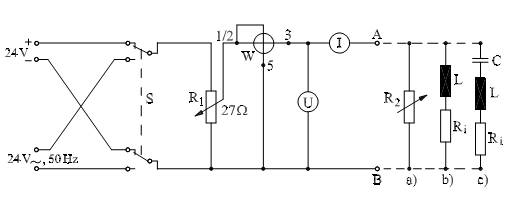
\includegraphics[width=0.7\textwidth]{Schaltplan.png}
	\caption{Schaltplan für die Aufgaben 4-8 \footcite{anleitung-ws2014}}
  \label{fig:kreisel1}
\end{figure}
In der zweiten Versuchsreihe wird die Zusammenhänge zwischen Spannung, Stromstärke und Leistung bei verschiedenen Bauteilen insbesondere bei Wechselstrom untersucht. Dazu wird eine Schaltung entsprechend Abbildung \ref{fig:kreisel1} aufgebaut bei der mithilfe des regelbaren Widerstandes $ R_1 $ verschiedene Spannungen angelegt werden können. Die Punkte $ A $ und $ B $ werden nacheinander durch verschiedene Verbraucher verbunden. Diese bestehen nacheinander aus einem ohmschen Widerstand, einem ohmschen Widerstand und einer Spule in Reihe, und einem ohmschen Widerstand, einer Spule und einem Kondensator in Reihe. Der ohmsche Widerstand im zweiten und dritten Verbraucher dient dabei der Vernachlässigung des Innenwiderstandes von Spule und Kondensator. Reguliert man nun die Spannung mittels $ R_1 $, so kann Stromstärke und Leistung in Abhängigkeit davon gemessen werden.
\subsection{Aufgabe 4}
Da es keine weiteren Angaben zur Frequenz der Wechselspannung gab, wurde von den normalen 50 Hz ausgegangen.

In dem Aufbau wird kein Verbraucher angeschlossen um die Verlustleistung des Voltmeters zu bestimmen. Diese beträgt bei maximaler Spannung, $U_{Gleich}=27V$ oder $U_{Wechsel}=25,5V$, $P_{verlust}=1W$ und nimmt bei sinkenden Spannungen weiter ab.
\subsection{Aufgabe 5}
An den Punkten A und B wird ein ohmscher Widerstand angeschlossen, für den bei Wechsel- und Gleichspannung die möglichen Messwerte bestimmt werden.
\begin{table}[H]
  \centering
  \begin{tabular}{c | c | c | c}
    Spannungsart & Spannung U [V] $\pm0,25$ & Stromstärke I [A] $\pm 0,05$ & Leistung P [W] $\pm0,5$\\ \hline
     & 24 & 1,00 & 23,7\\
     & 20 & 0,85 & 17,0\\
     Wechselspannung & 15 & 0,68 & 9,8\\
     & 10 & 0,43 & 4,0\\
     & 5 & 0,20 & 1,0\\ \hline
     & 25 & 1,00 & 24,5\\
     & 20 & 0,82 & 16,0\\
     Gleichspannung & 15 & 0,63 & 9,0\\
     & 10 & 0,42 & 3,9\\
     & 5 & 0,20 & 0,6
  \end{tabular}
  \caption{Messwerte des ohmschen Widerstands}
  \label{tab:messungohm}
\end{table}
\begin{figure}[H]
  \centering
  \begin{tikzpicture}
    \begin{axis}[
      width=15 cm,
      height=9 cm,
      xmin=0, xmax=30,
      ymin=0, ymax=1.2,
      xlabel={Angelenkte Spannung U [V]},
      ylabel={Gemessene Stromstärke I [A]},
      legend entries={Gleichspannung, Wechselspannung, Linearer Fit beider Spannungen},
      legend pos=north west,
      domain=0.1:28,
    ]
      \addplot plot [only marks,mark=x,thick,error bars/.cd, x dir=both, x fixed=0.25, y dir=both, y fixed=0.05]  file {GleichR.txt};
      \addplot plot [only marks,mark=o,thick,error bars/.cd, x dir=both, x fixed=0.25, y dir=both, y fixed=0.05]  file {WechselR.txt};
      \addplot[mark=none] {0.04*x+0.014};
    \end{axis}
  \end{tikzpicture}
  \caption{Versuch mit ohmschen Widerstand (Spannung gegen Stromstärke)}
  \label{fig:UIOhmscher}
\end{figure}
In dem Diagramm wurde nur der Fit für Gleichspannung eingetragen, da sich dieser fast mit dem von der Wechselspannung deckt und so eine größere Übersichtlichkeit erreicht wurde.

Aufgrund des anscheinend sehr linearen Verlaufs der Messwerte für beide Spannungsarten und in Deckung mit der zu erwarteten Formel \eqref{eq:Rohm} wurde mit \emph{gnuplot} nach dem \emph{least-squares}-Verfahren die Werte der beiden Spannungsarten gegen die Funktion $f(x)=m\cdot x$ gefittet. Ausgabe:
\begin{table}[H]
  \centering
  \begin{tabular}{c | c | c }
    Spannungsart & Variabel m  & Unsicherheit\\ \hline
    Gleichspannung & 0{,}040 & 0{,}002\\
    Wechselspannung & 0{,}042 & 0{,}003
  \end{tabular}
  \caption{Linearer Fit zu Abbildung \ref{fig:UIOhmscher}}
  \label{tab:fitUIOhmscher}
\end{table}
\begin{figure}[H]
  \centering
  \begin{tikzpicture}
    \begin{axis}[
      width=15 cm,
      height=9 cm,
      xmin=0, xmax=25,
      ymin=0, ymax=30,
      xlabel={Gemessene Leistung P [W]},
      ylabel={Produkt der Stromstärke I und der Spannung U [W]},
      legend entries={Gleichspannung, Wechselspannung, Linearer Fit beider Spannungen},
      legend pos=north west,
      domain=0.1:28,
    ]
      \addplot plot [only marks,mark=x,thick,error bars/.cd, x dir=both, x fixed=0.5, y dir=both, y fixed=0.5]  file {GleichR4.txt};
      \addplot plot [only marks,mark=o,thick,error bars/.cd, x dir=both, x fixed=0.5, y dir=both, y fixed=0.5]  file {WechselR2.txt};
      \addplot[mark=none] {1.005*x+0.352};
    \end{axis}
  \end{tikzpicture}
  \caption{Versuch mit ohmschen Widerstand (Leistung gegen Produkt aus Spannung und Stromstärke)}
  \label{fig:PUIOhmscher}
\end{figure}
In dem Diagramm wurde nur der Fit für Gleichspannung eingetragen, da sich dieser fast mit dem von der Wechselspannung deckt und so eine größere Übersichtlichkeit erreicht wurde. Der Fehler des Produktes von Stromstärke und Spannung wurde nach der Gaußschen Fehlerfortpflanzung bestimmt.

Aufgrund des anscheinend linearen Verlaufs der Messwerte für beide Spannungsarten und in Deckung mit der zu erwarteten Formel \ref{eq:leistung} wurde mit \emph{gnuplot} nach dem \emph{least-squares}-Verfahren die Werte der beiden Spannungsarten gegen die Funktion $f(x)=m\cdot x+b$ gefittet. Ausgabe:
\begin{table}[H]
  \centering
  \begin{tabular}{c | c | c | c}
    Spannungsart & Variabel m & Variabel b & Varians der Residuals\\ \hline
    Gleichspannung & 1,005 & 0,352 & 0,004\\
    Wechselspannung & 1,003 & 0,164 & 0,45
  \end{tabular}
  \caption{Linearer Fit zu Abbildung \ref{fig:PUIOhmscher}}
  \label{tab:fitPUIOhmscher}
\end{table}
\subsection{Aufgabe 6}
In diesem Versuchsteil wird eine Spule an den Punkten A und B angeschlossen (Aufbau b), und für Wechselspannung die Messwerte bestimmt.
\begin{table}[H]
  \centering
  \begin{tabular}{c | c | c}
    Spannung U [V] $\pm0,25$ & Stromstärke I [A] $\pm 0,05$ & Leistung P [W] $\pm0,5$\\ \hline
    25 & 0,85 & 16,2\\
    20 & 0,67 & 10,8\\
	15 & 0,50 & 6,0\\
    10 & 0,33 & 2,5\\
    5 & 0,20 & 1,0\\ 
  \end{tabular}
  \caption{Messwerte der Spule bei Wechselspannung}
  \label{tab:messungspulewechsel}
\end{table}
\begin{figure}[H]
  \centering
  \begin{tikzpicture}
    \begin{axis}[
      width=15 cm,
      height=9 cm,
      xmin=0, xmax=30,
      ymin=0, ymax=1.2,
      xlabel={Angelenkte Spannung U [V]},
      ylabel={Gemessene Stromstärke I [A]},
      legend entries={Wechselspannung, Linearer Fit},
      legend pos=north west,
      domain=0.1:28,
    ]
      \addplot plot [only marks,mark=x,thick,error bars/.cd, x dir=both, x fixed=0.25, y dir=both, y fixed=0.05]  file {WechselL.txt};
      
      \addplot[mark=none] {0.034*x-0.0096};
    \end{axis}
  \end{tikzpicture}
  \caption{Versuch mit Spule (Spannung gegen Stromstärke)}
  \label{fig:UISpule}
\end{figure}
\begin{table}[H]
  \centering
  \begin{tabular}{c | c | c | c}
    Spannungsart & Variabel m & Variabel b & Varians der Residuals\\ \hline
    Wechselspannung & 0,034 & -0,0096 & $2,54\cdot10^{-5}$
  \end{tabular}
  \caption{Linearer Fit zu Abbildung \ref{fig:UISpule}}
  \label{tab:fitUISpule}
\end{table}
\begin{figure}[H]
  \centering
  \begin{tikzpicture}
    \begin{axis}[
      width=15 cm,
      height=9 cm,
      xmin=0, xmax=20,
      ymin=0, ymax=25,
      xlabel={Leistung P [W]},
      ylabel={Produkt der Stromstärke I und der Spannung U [W]},
      legend entries={Wechselspannung, Linearer Fit},
      legend pos=north west,
      domain=0.1:28,
    ]
      \addplot plot [only marks,mark=x,thick,error bars/.cd, x dir=both, x fixed=0.5, y dir=both, y fixed=0.5]  file {WechselL2.txt};
      
      \addplot[mark=none] {1.301*x-0.171};
    \end{axis}
  \end{tikzpicture}
  \caption{Versuch mit Spule (Leistung gegen Produkt aus Spannung und Stromstärke)}
  \label{fig:PUISpule}
\end{figure}
Der Fehler des Produktes von Stromstärke und Spannung wurde nach der Gaußschen Fehlerfortpflanzung bestimmt.
\begin{table}[H]
  \centering
  \begin{tabular}{c | c | c | c}
    Spannungsart & Variabel m & Variabel b & Varians der Residuals\\ \hline
    Wechselspannung & 1,301 & -0,171 & 0,14
  \end{tabular}
  \caption{Linearer Fit zu Abbildung \ref{fig:PUISpule}}
  \label{tab:fitPUISpule}
\end{table}
Aus dem Fit \ref{tab:fitPUISpule} ergibt sich, wenn man den $b$ Achsenabschnitt, der aus Messungenauigkeiten folgt, vernachlässigt,
\begin{equation}
U\cdot I=1,301\cdot P.
\end{equation}
Wenn man dies nun in \eqref{eq:phase} einsetzt und nach dem Phasenwinkel $\varphi$ auflöst, erhält man
\begin{equation}
\varphi = \pm \arccos\left(\frac{1}{1{,}301}\right) \approx \pm 39{,}77^\circ.
\end{equation}
Da es sich um eine Schaltung bestehend aus nur einer Spule handelt, kann man allgemein sagen, dass die Stromstärke der Spannung folgt, woraus folgt, dass gilt
\begin{equation}
\varphi = 39,77^\circ.
\end{equation}

Aus dem Fit \ref{tab:fitUISpule} ergibt sich unter der Vernachlässigung von b
\begin{equation}
I=0,034\Omega^{-1}\cdot U.
\end{equation}
Wenn man dies nun in die Formel \eqref{eq:wirkohm} einsetzt erhält man
\begin{equation}
R_W=\frac{U}{I}\cos(\varphi)=\frac{U}{0,034\Omega^{-1}\cdot U}\cos(\varphi)=\frac{1}{0,034\Omega^{-1}}\cos(\varphi)= \frac{500}{17}\cos(\varphi)\Omega \approx 22,61 \Omega
\end{equation}
\subsection{Aufgabe 7}
In diesem Versuchsteil wird bei gleichem Aufbau wie in Aufgabe 6 eine Gleichspannung angelegt. Da der Wirkwiderstand der Spule bei Gleichstrom 0 wird, kann so der Innenwiderstand der Spule bestimmt werden.
\begin{table}[H]
  \centering
  \begin{tabular}{c | c }
    Spannung U [V] $\pm0,25$ & Stromstärke I [A] $\pm 0,05$ \\ \hline
    24,5 & 1,0 \\
    19,0 & 0,8\\
	14,0 & 0,6 \\
    9,1 & 0,4 \\
    5,0 & 0,2 \\ 
  \end{tabular}
  \caption{Messwerte der Spule bei Wechselspannung}
  \label{tab:messungspulegleich}
\end{table}
\begin{figure}[H]
  \centering
  \begin{tikzpicture}
    \begin{axis}[
      width=15 cm,
      height=9 cm,
      xmin=0, xmax=30,
      ymin=0, ymax=1.2,
      xlabel={Angelenkte Spannung U [V]},
      ylabel={Gemessene Stromstärke I [A]},
      legend entries={Gleichspannung, Linearer Fit},
      legend pos=north west,
      domain=0.1:28,
    ]
      \addplot plot [only marks,mark=x,thick,error bars/.cd, x dir=both, x fixed=0.25, y dir=both, y fixed=0.05]  file {GleichL.txt};
      
      \addplot[mark=none] {0.041*x+0.016};
    \end{axis}
  \end{tikzpicture}
  \caption{Versuch mit Spule}
  \label{fig:UIGleichSpule}
\end{figure}
\begin{table}[H]
  \centering
  \begin{tabular}{c | c | c | c}
    Spannungsart & Variabel m & Variabel b & Varians der Residuals\\ \hline
    Gleichspannung & 0,041 & 0,016 & 0,00035
  \end{tabular}
  \caption{Linearer Fit zu Abbildung \ref{fig:UIGleichSpule}}
  \label{tab:fitUIGleichSpule}
\end{table}
Aus dem Fit \ref{tab:fitUIGleichSpule} ergibt sich unter der Vernachlässigung von b
\begin{equation}
I=0,041\Omega^{-1}\cdot U.
\end{equation}
Wenn man dies nun in die Formel \ref{eq:Rohm} einsetzt erhält man
\begin{equation}
R_i=\frac{U}{I}=\frac{U}{0,041\Omega^{-1}\cdot U}=\frac{1}{0,041\Omega^{-1}}= \frac{1000}{41}\Omega = 24,\overline{39024} \Omega
\end{equation}
Aus der Formel \eqref{eq:Induk} folgt
\begin{equation}
L=\sqrt{\frac{|Z|^2-R^2}{\omega^2}}\approx 0,052~\si{\henry}
\end{equation}
\subsection{Aufgabe 8}
In diesem Versuchsteil wird zusätzlich ein Kondensator in Reihe geschaltet. Daraufhin wird Wechselspannung angelegt, und die Stromstärke und Leistung abhängig davon gemessen.
\begin{figure}[H]
  \centering
  \begin{tikzpicture}
    \begin{axis}[
      width=15 cm,
      height=9 cm,
      xmin=0, xmax=30,
      ymin=0, ymax=0.65,
      xlabel={Angelenkte Spannung U [V]},
      ylabel={Gemessene Stromstärke I [A]},
      legend entries={Wechselspannung, Linearer Fit},
      legend pos=north west,
      domain=0.1:28,
    ]
      \addplot plot [only marks,mark=x,thick,error bars/.cd, x dir=both, x fixed=0.25, y dir=both, y fixed=0.05]  file {WechselLC.txt};
      
      \addplot[mark=none] {0.0229*x+0.00344};
    \end{axis}
  \end{tikzpicture}
  \caption{Versuch mit Spule und Kondensator (Spannung gegen Stromstärke)}
  \label{fig:UILC}
\end{figure}
\begin{table}[H]
  \centering
  \begin{tabular}{c | c | c | c}
    Spannungsart & Variabel m & Variabel b & Varians der Residuals\\ \hline
    Wechselspannung & 0,023 & 0,003 & $1,36\cdot10^{-5}$
  \end{tabular}
  \caption{Linearer Fit zu Abbildung \ref{fig:UILC}}
  \label{tab:fitUILC}
\end{table}
\begin{figure}[H]
  \centering
  \begin{tikzpicture}
    \begin{axis}[
      width=15 cm,
      height=9 cm,
      xmin=0, xmax=10,
      ymin=0, ymax=15,
      xlabel={Leistung P [W]},
      ylabel={Produkt der Stromstärke I und der Spannung U [W]},
      legend entries={Wechselspannung, Linearer Fit},
      legend pos=north west,
      domain=0:9,
    ]
      \addplot plot [only marks,mark=x,thick,error bars/.cd, x dir=both, x fixed=0.5, y dir=both, y fixed=0.5]  file {WechselLC2.txt};
      
      \addplot[mark=none] {1.62*x+0.27};
    \end{axis}
  \end{tikzpicture}
  \caption{Versuch mit Spule(Leistung gegen Produkt aus Spannung und Stromstärke)}
  \label{fig:PUILC}
\end{figure}
Der Fehler des Produktes von Stromstärke und Spannung wurde nach der Gaußschen Fehlerfortpflanzung bestimmt.
\begin{table}[H]
  \centering
  \begin{tabular}{c | c | c | c}
    Spannungsart & Variabel m & Variabel b & Varians der Residuals\\ \hline
    Wechselspannung & 1,62 & 0.27 & 0,038
  \end{tabular}
  \caption{Linearer Fit zu Abbildung \ref{fig:PUILC}}
  \label{tab:fitPUILC}
\end{table}
Der Phasenwinkel lässt sich analog zu Aufgabe 6 berechnen
\begin{equation}
\varphi=arccos(1,62^{-1})=51,88^{\circ}.
\end{equation}
Ebenso kann man den Widerstand |Z| so wie bei Aufgabe 6 berechnen.
\begin{equation}
|Z|=\frac{1}{0,023\Omega^{-1}}=\frac{1000}{23}\Omega\approx 43,48\Omega
\end{equation}

Damit kann nun die Kapazität des Kondensators berechnet werden
\begin{equation}
C=\frac{1}{\omega^2L+\omega\sqrt{|Z|^2-R^2}}=\SI{60.72}{\micro\farad}
\end{equation}
\section{Diskussion}
\subsection{Versuchsreihe 1}
Im ersten Versuch wurde überprüft, ob das Modell des Innenwiderstandes das reale Verhalten eines Akkumulators als Spannungsquelle gut beschreiben kann. Der offensichtlich lineare Zusammenhang in \cref{fig:fita1} bestätigt dies für alle drei Messreihen.
Allerdings wurde im Versuch ein Vorwiderstand vor den Akku geschaltet, um den Effekt deutlicher sichtbar zu machen. Anhand des Farbcodes wurde ermittelt, dass dieser bei $R_V=\SI{18}{\ohm}\pm \SI{1}{\percent}$ liegt. Die relative Abweichung zum gemessenen Innenwiderstand beträgt
\begin{itemize}
  \item Für eine Zelle: $(\SI{18}{\ohm}-\SI{17.2}{\ohm})/\SI{18}{\ohm}\approx \SI{4.4}{\percent}$
  \item Für drei Zellen parallel: $(\SI{18}{\ohm}-\SI{44.9/3}{\ohm})/\SI{18}{\ohm}\approx \SI{16.85}{\percent}$
  \item Für drei Zellen in Reihe: $(\SI{18}{\ohm}-\SI{15.6}{\ohm})/\SI{18}{\ohm}\approx \SI{13.3}{\percent}$
\end{itemize}
Es fällt auf, dass die gemessenen Innenwiderstände systematisch unterhalb des erwarteten Wertes liegen. Das Modell scheint also die Realität bei einer Zelle sehr gut zu beschreiben, während es bei mehreren Zellen ungenauer wird. \\

Die an den Verbraucher abgegebene Leistung scheint nach \cref{fig:leistunga2} sehr gut durch den Zusammenhang aus \cref{eq:leistung} beschrieben zu werden. Da der Graph der Funktion aus \cref{eq:leistung} sehr gut mit den Messpunkten übereinstimmt, liegt auch das Maximum der Leistung beim berechneten Außenwiderstand $R_a=R_i$.
\subsection{Versuchsreihe 2}
Zumindest qualitativ ließen sich in allen Versuchsteilen die theoretisch ermittelten Zusammenhänge zeigen. Bei jeder Messreihe ließ sich Spannung gegen Stromstärke sowie Produkt aus Spannung und Stromstärke ohne Ausreißer und ohne größere Fehler linear gegeneinander Auftragen. Jedoch Fehlen bei den meisten Ergebnissen die Referenzwerte um festzustellen, ob die Werte auch qualitativ passen. Der einzige gegebene Referenzwert, die Kapazität des Kondensators, stimmt jedoch sehr gut mit unseren Ergebnissen überein. Der von uns bestimmte Wert $ \SI{60.72}{\micro\farad} $ weicht von dem angegebenen Wert nur um etwas mehr als $ \SI{1}{\percent} $ ab. Dennoch könnte dieses gute Ergebnis durch mehrere sich aufhebende Fehler begünstigt sein.
\notecite{anleitung-ws2014}
